\chapter{Fokusgruppe}

In dieser Fokusgruppe wurde untersucht, wie Datenbrillen von Handwerkern aufgenommen werden und ob diese sich Szenarien vorstellen können, in welchen der Einsatz von Datenbrillen in ihrem Arbeitsumfeld hilfreich ist. Die Ursprüngliche Idee war dabei, dass Datenbrillen zur Unterstützung von Handwerkern eingesetzt werden, beispielsweise in Fernwartungsszenarien, wenn eine Person sehen möchte, was eine andere Person sieht, sich diese aber nicht am selben Ort befinden. Dann kann das Bild von der Brille des einen, zum Monitor des anderen übertragen werden. \\
Im Folgenden werden dazu die Rahmenbedingungen und die Intention, die Durchführung, sowie die Auswertung der geäußerten Ideen beschrieben. Dabei kristallisierten sich zwei Anwendungsbereiche für AR heraus, die genauer beleuchtet werden, da sie zum weiteren Verlauf dieser Forschung beitragen.

\begin{figure}[h]
	\begin{center}
		\noindent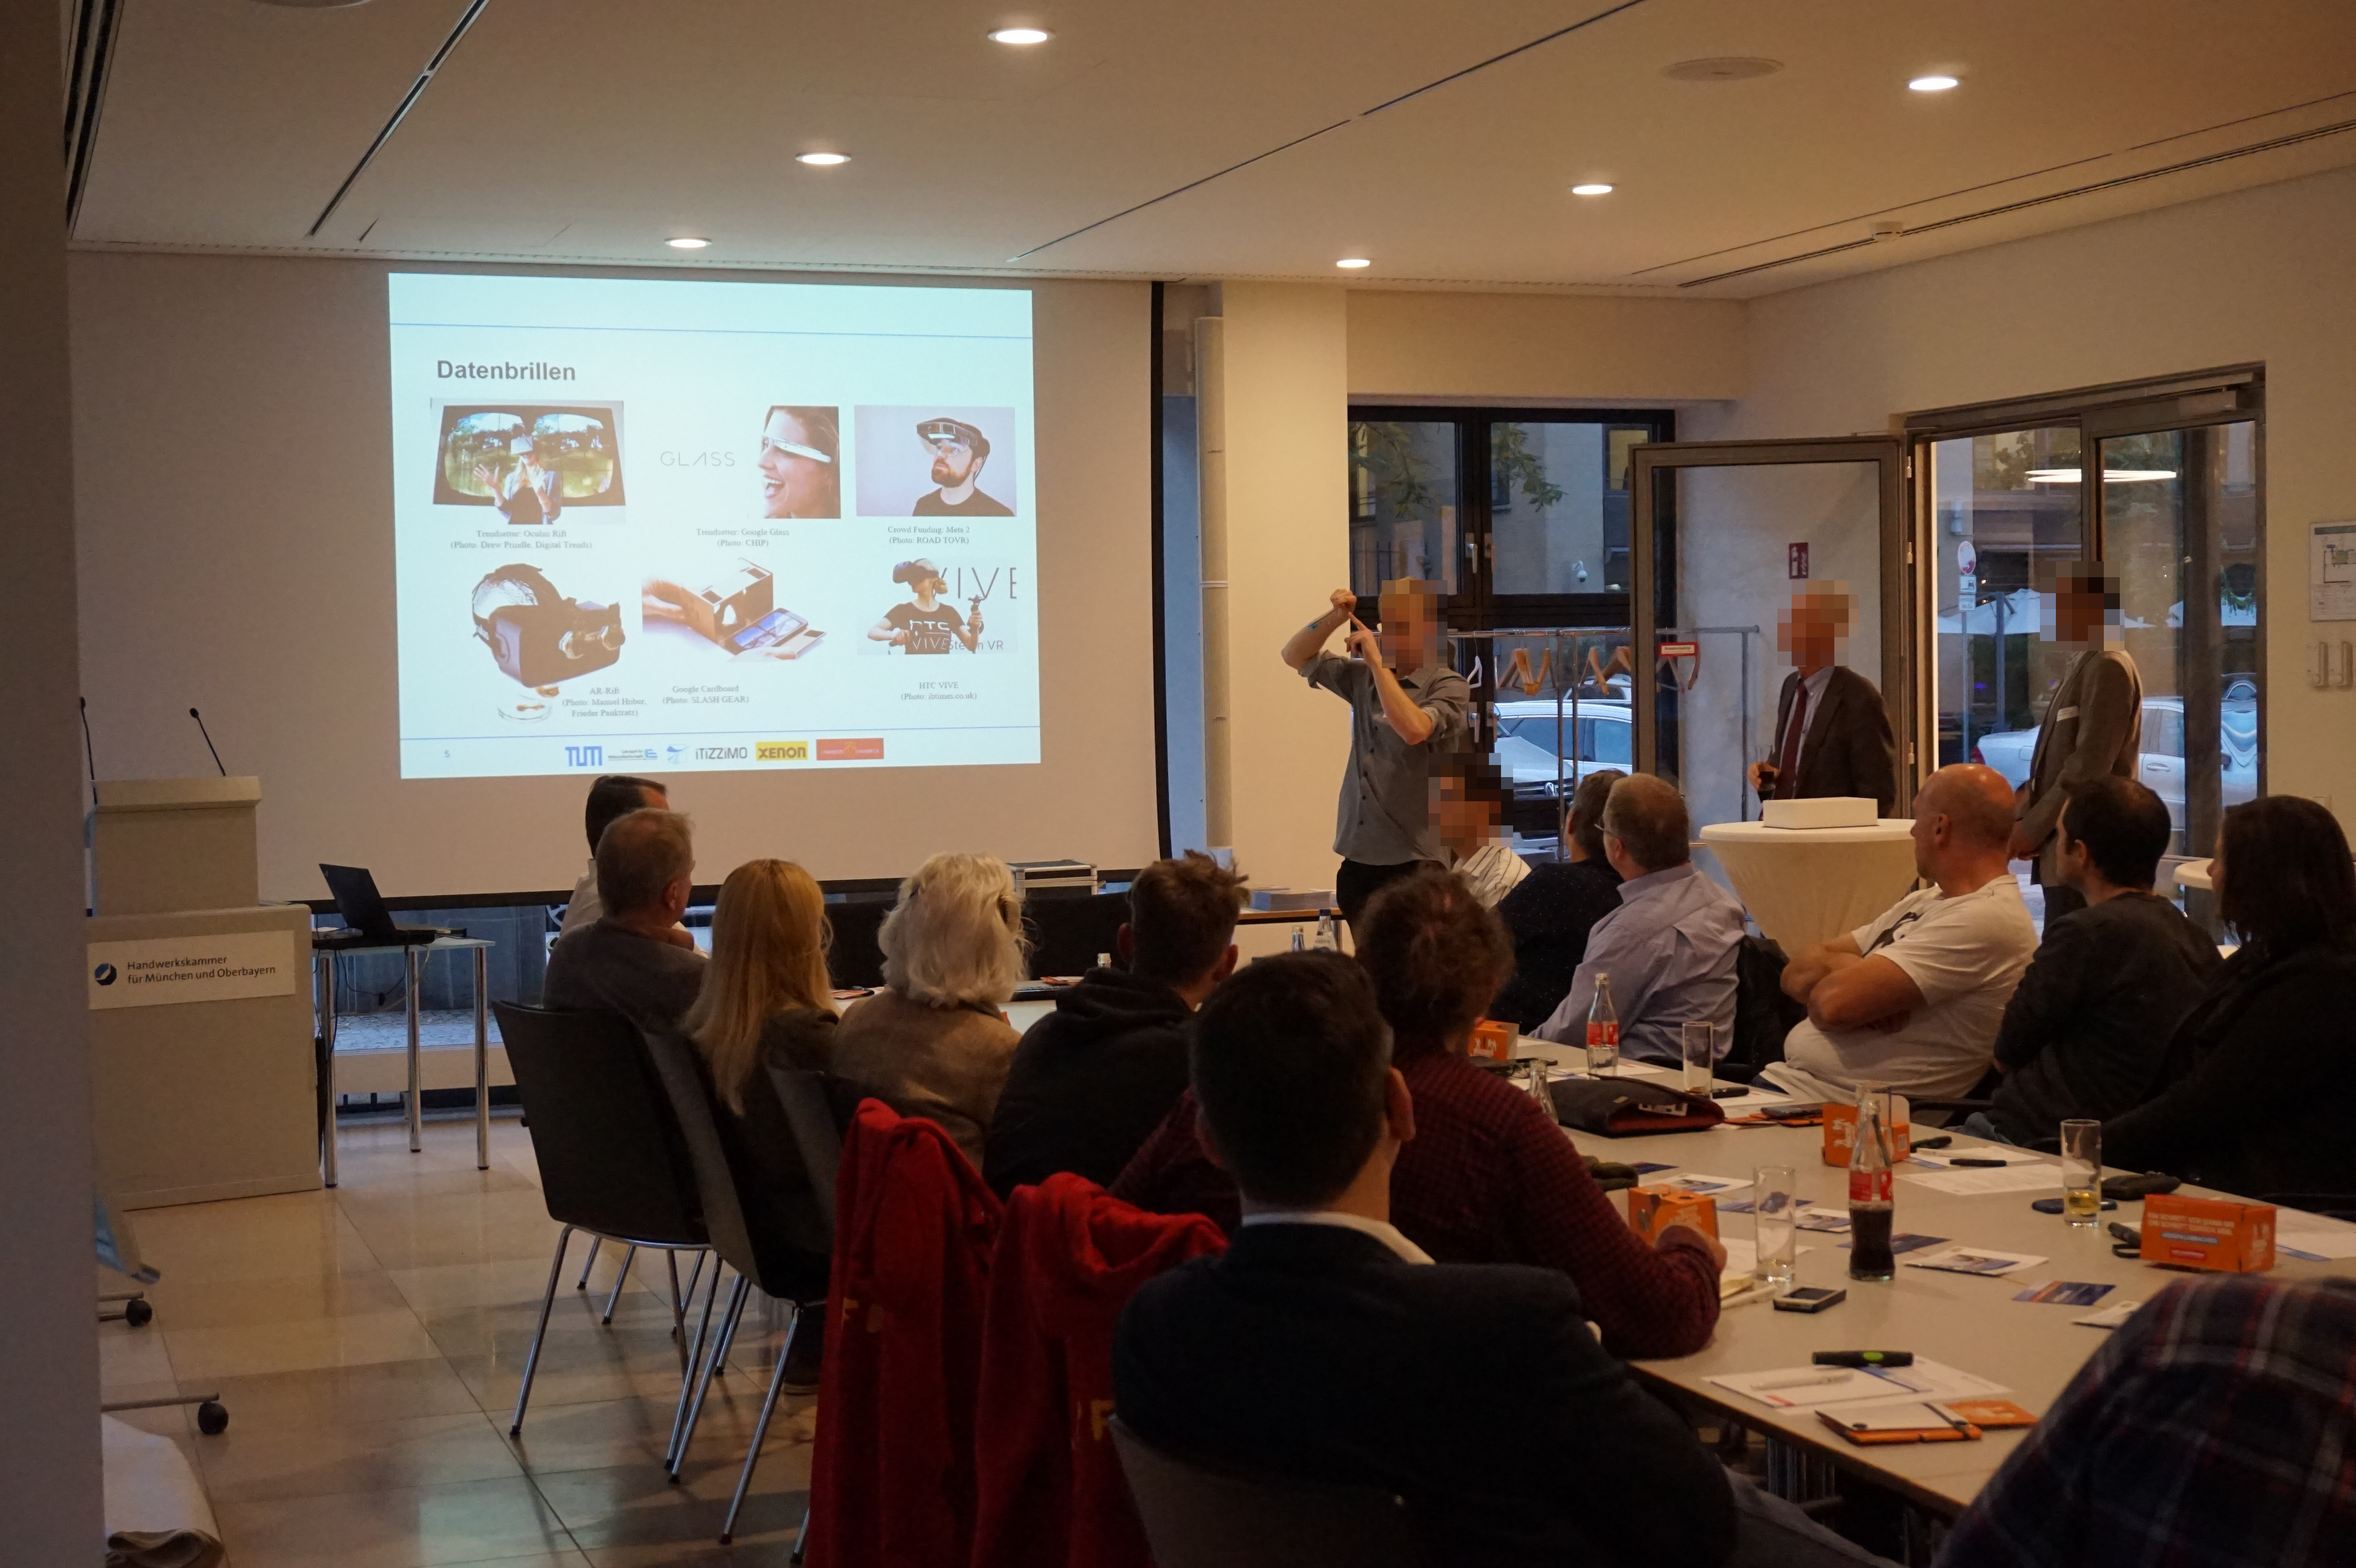
\includegraphics[width=\linewidth,height=\textheight,keepaspectratio]{Resources/Fokusgruppe_pres.jpg}
		\caption{Präsentation der Datenbrillen und Anwendungsbeispiele}
	\end{center}
\end{figure}

\section{Rahmen}

Um ein generelles Bild der Akzeptanz von Augmented Reality im Handwerk zu prüfen, wurde eine Fokusgruppe dazu in der Handwerkskammer München organisiert. Dazu wurden ca. 20 Handwerker aus verschiedenen handwerklichen Branchen eingeladen, um über das Thema zu diskutieren. Anfangs hielt der Moderator einen Vortrag über Augmented Reality allgemein, um den Teilnehmern die Technologie näher zu bringen. Anschließend standen verschiedene Datenbrillen, wie zum Beispiel Google Glass und die Microsoft HoloLens (siehe Abbildung \ref{datenbrillen}), zur Verfügung, welche von den Teilnehmern ausprobiert werden konnten. Die Forschungsfragen für den Workshop waren: "Was denken Handwerker über Augmented Reality, speziell Datenbrillen?" und "Können sich Handwerker Szenarien vorstellen, für welche der Einsatz von Datenbrillen für sie sinnvoll wäre?". Diese gab der Moderator den Testpersonen mit für das Testen der Brillen.

\begin{figure}[h]
	\begin{center}
		\noindent\includegraphics[width=\linewidth,height=\textheight,keepaspectratio]{Resources/Datenbrillen.jpg}
		\caption{Datenbrillen}
		\label{datenbrillen}
	\end{center}
\end{figure}

\section{Testen der Brillen}

Für jede Brille wurde eine eigene Station aufgebaut. Das Augenmerk dieser Arbeit liegt auf der Microsoft HoloLens, da dieses die am weitesten fortgeschrittene Technologie ist. Es handelt sich dabei um eine große Brille, welche mit Kameras, die ihre Umgebung filmt, sowie Mikrofon und Lautsprechern ausgestattet ist. Sie erlaubt es im Sichtfeld des Nutzers Hologramme anzuzeigen und mit diesen zu interagieren. Dieser sieht dabei die "reale Welt", welche durch die Hologramme erweitert wird. In der Fachliteratur wird dies als \textbf{Augmented Reality} oder \textbf{Mixed Reality} bezeichnet, da es reale und virtuelle Welt verschmilzt.

\begin{figure}[h]
	\begin{center}
		\noindent\includegraphics[width=\linewidth,height=\textheight,keepaspectratio]{Resources/Fokusgruppe2.jpg}
		\caption{Testen der Brillen durch Handwerker}
	\end{center}
\end{figure}

Das Szenario, welches mit der HoloLens nachgespielt wurde, orientierte sich an der oben genannten ursprünglichen Idee. Dies wurde mit der Applikation Skype für HoloLens und PC nachgestellt. Die Skype Applikation für HoloLens ermöglicht es dem Nutzer mit anderen über das Internet zu telefonieren. Der Nutzer sieht dabei die Webcamübertragung seines Gesprächspartners in einem Fenster-Hologramm, welches er in seiner Umgebung positionieren kann und hört diesen über die Lautsprecher der Brille. Der Nutzer am Computer sieht einen Livestream der Aufnahmen der HoloLens. Er sieht also auch Hologramme, die dieser im Raum positioniert. Beide Kommunikationspartner können mit dem Livestream und dadurch miteinander interagieren. Sie können Pfeile einzeichnen, oder Bilder in der Umgebung des HoloLensträgers platzieren. 

So ist es beispielsweise für den Brillenträger möglich dem Computernutzer ein Problem zu zeigen. Dieser kann ihn aus der Ferne beim Lösen assistieren, was in einem Laien-Experten Szenario hilfreich sein kann. Der Computernutzer erhält so einen guten Einblick in das Problem und direktes Feedback zu den Aktionen des Brillenträgers und seinen Anweisungen. Dadurch können sie sich besser abstimmen.

\section{Diskussionsrunde}

\begin{figure}[h]
	\begin{center}
		\noindent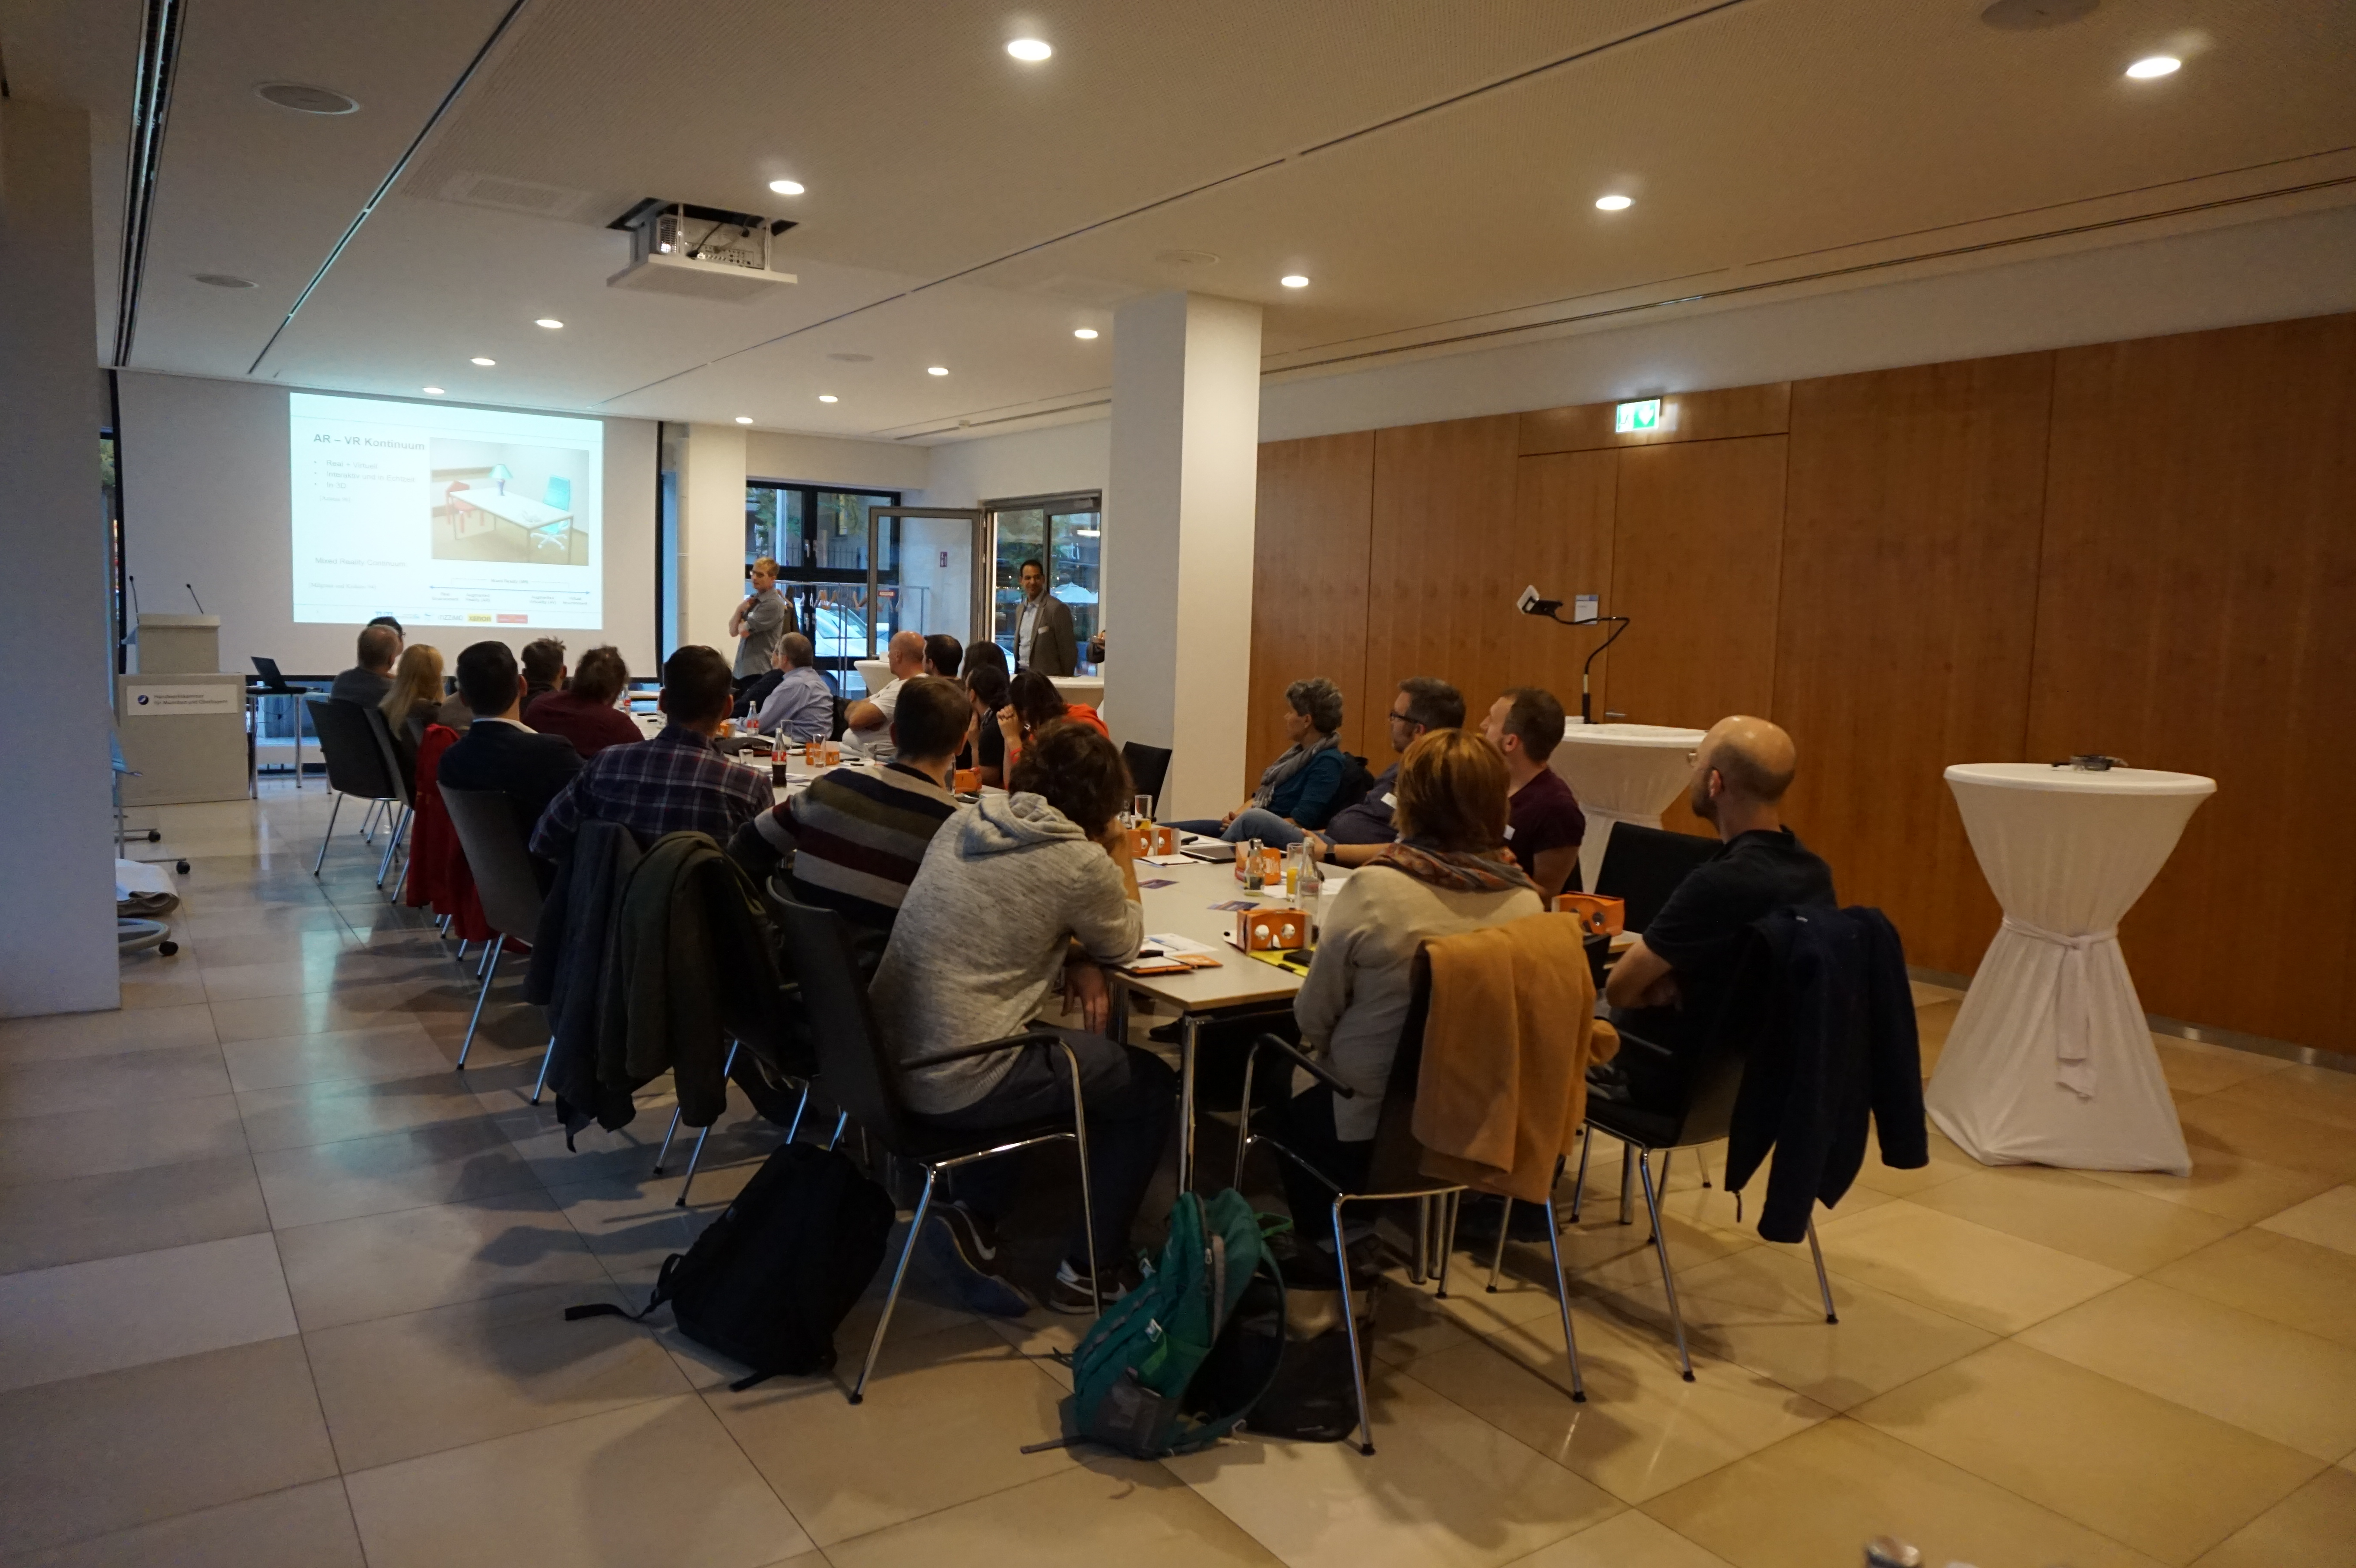
\includegraphics[width=\linewidth,height=\textheight,keepaspectratio]{Resources/Fokusgruppe1.jpg}
		\caption{Diskussion in der Fokusgruppe}
	\end{center}
\end{figure}

Die Diskussionsrunde wurde an einer langen Tafel abgehalten. Der Moderator stellte noch einige Applikationen und Anwendungsmöglichkeiten von Augmented Reality vor, um die Fantasie der Teilnehmer anzuregen. Danach stellte er richtungsweisende Fragen, was die Diskussion anregte. Dabei kristallisierten sich schnell zwei gefragte Themenbereiche heraus: Augmented Reality als Assistent für den Handwerker zu nutzen, der ihn bei der Ausführung seiner Arbeit unterstützt und es als visuelles Tool für das Kundengespräch zu nutzen. Die meisten Ideen drehten sich um diese Anwendungsmöglichkeiten. Zusätzlich wurde aber auch Kritik an der Microsoft HoloLens geäußert, warum sie eventuell nicht genutzt werden kann.

\subsection{Kritik an dem Einsatz von Augmented Reality und der Microsoft HoloLens}

Es wurden die hohen Anschaffungskosten kritisiert, die mit dem kauf der Microsoft HoloLens einhergehen. Diese kostet momentan ca. 3000\EURdig, was ein großer Aufwand für einen kleinen Handwerksbetrieb wäre. Dazu braucht der Handwerker auch die richtige Software, welche noch auf seine Bedürfnisse zugeschnitten werden muss. Da Teilnehmer äußerten hierzu Bedenken, dass der Kosten/Nutzen Faktor für sie nicht Interessant sein könnte.

Für das Beispiel mit Skype wurden die Bedenken geäußert, dass man dafür eine ständige, stabile Internetverbindung benötigt. Diese ist oft auf einer Baustelle oder einer großen Produktionshalle nicht gegeben. Dadurch könnten Fernwartungsapplikationen nicht verwendet werden.

Ein großer Kritikpunkt ist die Einsatzfähigkeit der HoloLens auf einer Baustelle. Dieses Umfeld ist hart, schmutzig, staubig und oft ungemütlich. Man findet schwer einen sicheren Platz zum abstellen der Brille. Bei jedem hinlegen läuft man Gefahr diese zu zerkratzen oder anderweitig zu beschädigen. Noch dazu hält sie wahrscheinlich keinen harten Stößen stand, falls sie herunterfallen sollte. Der Staub auf Baustellen kann sich negativ auf die Funktionalität der Kameras und die Darstellung der Hologramme auswirken. Gegebenenfalls erkennt die Brille dadurch die Gestensteuerung nicht mehr. Zusätzlich ist die Microsoft HoloLens ein eher unhandliches, globiges Gerät, welches man auf dem Kopf trägt. Das beeinflusst die Komfortabilität der Nutzung der Brille, vor allem bei längerem Gebrauch.

\subsection{AR als Assistent für den Handwerker}

Oft wurde von den Handwerkern der Wert einer Funktion zum automatischen Erfassen des Raumes hervorgehoben. Der initiale Prozess zum Abmessen der Wandlängen, Winkel, Einbuchtungen und sonstigem nimmt einiges an Zeit in Anspruch. Gleichzeitig handelt es sich dabei um einen wichtig Schritt, der den Grundstein für das weitere Vorgehen legt. Jeder Handwerker, sei es Fliesenleger, Maurer oder Installateur benötigt diese Daten für die Planung. Mit Augmented Reality kann es möglich sein, dies automatisch zu erfassen. Die Microsoft HoloLens beispielsweise besitzt ein integriertes \textbf{spacial mapping}, mithilfe dessen sich die Brille ein Verständnis der Umgebung verschafft. Diese Funktionalität könnte dafür genutzt werden eine solche Applikation zu integrieren. 

Nach dem erfassen des Raumes ist es für Handwerker interessant verschiedene Objekte, wie zum Beispiel Fliesen, Lampen, Fenster, Waschbecken oder ähnliches virtuell im Raum platzieren zu können. Das erleichtert die Planung, da man bereits in diesem Schritt festlegen kann, wie das Endergebnis aussieht und dadurch abschätzen kann wie viel Material benötigt wird. Das Material richtig abzuschätzen ist ein Problem, welches Handwerkern immer wieder begegnet. Zusätzlich äußerte ein Installateur die Idee, dass die Brille Verstöße gegen DIN Normen, wie beispielsweise die Höhe von Treppenstufen oder Toiletten direkt anzeigt und somit den Raum für Fehler minimiert. 

Die Datenbrille kann so also als Planungswerkzeug für den Handwerker verwendet werden. Dadurch hat er den Plan direkt vor Augen und kann ihn gegebenenfalls mit anderen Handwerkern teilen. Dies ist besonders interessant, wenn beispielsweise ein Handwerker das Kundengespräch leitet und den entstandenen Plan mit seinen Mitarbeitern teilen möchte. So kann sichergestellt werden, dass alle auf das gleiche Endergebnis hinarbeiten. Traditionell, äußerten einige Teilnehmer der Fokusgruppe, wird das oft über Telefonate abgestimmt. Dabei kommt es leicht zu Missverständnissen und somit zu Fehlern bei der Umsetzung. Eine visuelle Darstellung würde das Telefonat unterstützen und ein verständlicheres Bild zeichnen.

\subsection{AR als Assistent für das Kundengespräch}

Ein großes Problem aller Handwerker stellt das Kundengespräch dar. Sie kritisieren, dass Kunden kaum Vorstellungskraft haben. Der Handwerker kann sich das Ergebnis seiner Arbeit in einem unfertigen Raum leichter vorstellen, als der Kunde, welcher meist Laie auf dem Gebiet ist. Eine visuelle Darstellung des Plans durch Hologramme kann von diesen leichter verstanden werden, als beispielsweise ein technischer Bauplan. 

Diese visuelle Darstellung unterstützt auch beim Austausch mit dem Kunden. Dieser kann direkt sehen, wie der Handwerker seine Wünsche verstanden hat und so leichter Änderungen vorschlagen. Dadurch lassen sich Änderungswünsche, welche im späteren Verlauf der Arbeit beim Kunden auftreten könnten minimieren. Generell kann dadurch die Ambiguität in Kundengesprächen verringert werden, was eine höhere Planungssicherheit gewährleistet. 

Auch der Handwerker kann dem Kunden damit seine Vorschläge besser vor Augen führen. Die Handwerker merkten an, dass der Kunde sich oft nichts unter den Vorschlägen des Experten vorstellen kann. So werden diese ihm direkt visuell vorgeführt. Das erhöht gleichzeitig das Vertrauen in den Handwerker, da bereits beim Betrachten des Plans deutlich wird, dass DIN Normen eingehalten wurden und riskante Designs ersichtlich sind. 

Außerdem unterstützt es auch bei dem Vertragsschluss. Alle umzusetzenden Aspekte sind visuell erfassbar und dadurch digital dokumentiert. Damit lassen sich diese sehr gut im Vertrag festhalten. Es ist also für den Kunden sichergestellt, dass der Handwerker genau nach Plan vorgeht. Für den Handwerker hingegen lassen sich so Änderungen, welche vom Kunden nach der eigentlichen Vertragsschließung gefordert werden gut abgrenzen und als zusätzliche Leistungen abrechnen. 

\section{Fazit}

Ein AR Raumplaner hat, wie durch die Fokusgruppe deutlich geworden, einige Anwendungsszenarien und wird von Handwerkern gewünscht. Generell waren die Handwerker von der Technologie Augmented Reality sehr begeistert, was sich an den vielen eingebrachten Ideen zeigt. Der allgemeine Konsensus zeigt dabei auch in eine deutliche Richtung. Die ursprüngliche Idee zur Unterstützung in Fernwartungsszenarien fand nicht so viel Anklang. Handwerker interessieren sich eher für Unterstützung durch AR bei Tätigkeiten wie Maße nehmen und Planen. Auch eine visuelle Hilfe bei Kundengesprächen stellt sich als durchaus benötigt heraus. 

Allerdings wird es noch dauern, bis die Technologie ausgereift genug ist, um den Genauigkeitsansprüchen zu genügen. Die Geräte müssten für den Bau auch robuster designt und gebaut werden, um den harten Bedingungen zu trotzen. 

Zusammenfassen lässt sich jedoch sagen, dass die Datenbrillen von den Handwerkern gut akzeptiert wurden und diese Potential für die Zukunft dieser im Handwerk sehen. \\
Um diesen Ansätzen weiter nachzugehen muss tiefer in die Materie eingestiegen werden. Der Beruf eines Handwerkers muss aus der Nähe untersucht werden, um herauszufinden, wo man mit einer Applikation unterstützen kann, und ob man diese in den Arbeitsalltag eines Handwerkers integrieren kann. 

Der Beruf des Fliesenlegers würde dabei einige Aspekte abdecken. Ein Raum muss ausgemessen und darin Objekte - Fliesen - verlegt werden. Das lässt sich für Microsoft HoloLens gut umsetzen. Daher wird im nächsten Kapitel eine Ethnographie zum Beruf des Fliesenlegers angefertigt, mit dem Ziel definitive Ansatzpunkte für eine Applikation zur Unterstützung von Handwerkern, im speziellen Fliesenleger, zu erstellen.